% Created by tikzDevice version 0.10.1 on 2017-11-07 14:46:43
% !TEX encoding = UTF-8 Unicode
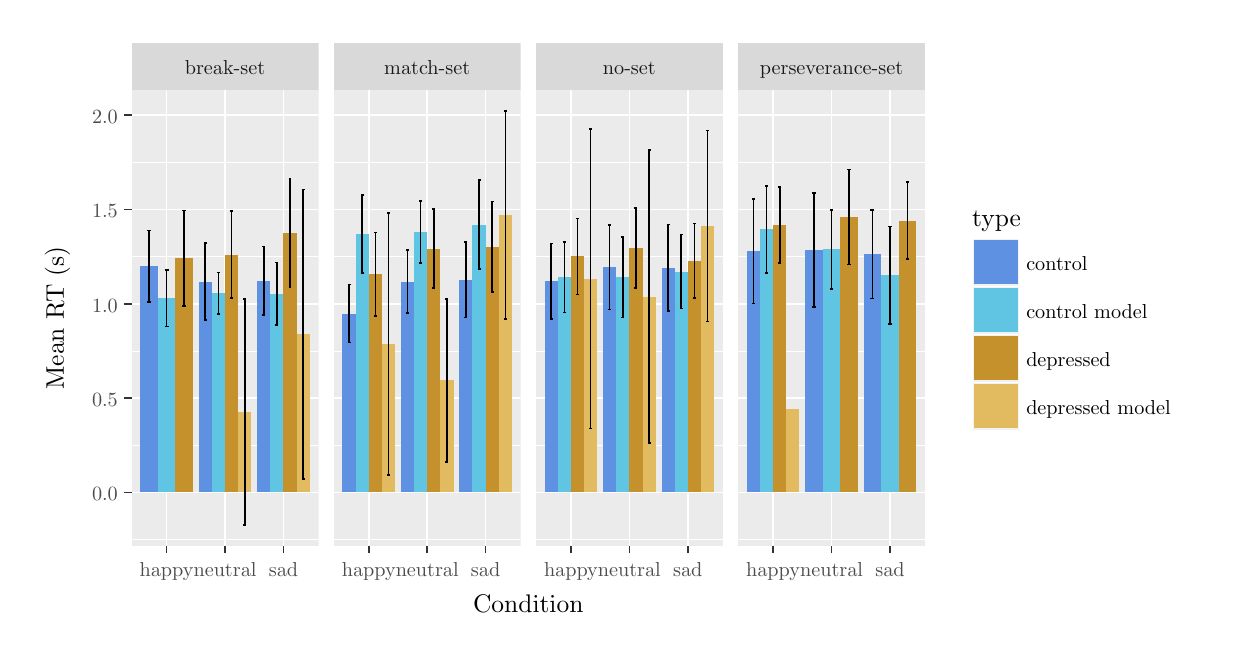
\begin{tikzpicture}[x=1pt,y=1pt]
\definecolor{fillColor}{RGB}{255,255,255}
\path[use as bounding box,fill=fillColor,fill opacity=0.00] (0,0) rectangle (433.62,216.81);
\begin{scope}
\path[clip] (  0.00,  0.00) rectangle (433.62,216.81);
\definecolor{drawColor}{RGB}{255,255,255}
\definecolor{fillColor}{RGB}{255,255,255}

\path[draw=drawColor,line width= 0.6pt,line join=round,line cap=round,fill=fillColor] (  0.00,  0.00) rectangle (433.62,216.81);
\end{scope}
\begin{scope}
\path[clip] ( 37.53, 29.59) rectangle (105.09,194.25);
\definecolor{fillColor}{gray}{0.92}

\path[fill=fillColor] ( 37.53, 29.59) rectangle (105.09,194.25);
\definecolor{drawColor}{RGB}{255,255,255}

\path[draw=drawColor,line width= 0.3pt,line join=round] ( 37.53, 31.85) --
	(105.09, 31.85);

\path[draw=drawColor,line width= 0.3pt,line join=round] ( 37.53, 65.92) --
	(105.09, 65.92);

\path[draw=drawColor,line width= 0.3pt,line join=round] ( 37.53,100.00) --
	(105.09,100.00);

\path[draw=drawColor,line width= 0.3pt,line join=round] ( 37.53,134.07) --
	(105.09,134.07);

\path[draw=drawColor,line width= 0.3pt,line join=round] ( 37.53,168.15) --
	(105.09,168.15);

\path[draw=drawColor,line width= 0.6pt,line join=round] ( 37.53, 48.88) --
	(105.09, 48.88);

\path[draw=drawColor,line width= 0.6pt,line join=round] ( 37.53, 82.96) --
	(105.09, 82.96);

\path[draw=drawColor,line width= 0.6pt,line join=round] ( 37.53,117.04) --
	(105.09,117.04);

\path[draw=drawColor,line width= 0.6pt,line join=round] ( 37.53,151.11) --
	(105.09,151.11);

\path[draw=drawColor,line width= 0.6pt,line join=round] ( 37.53,185.19) --
	(105.09,185.19);

\path[draw=drawColor,line width= 0.6pt,line join=round] ( 50.20, 29.59) --
	( 50.20,194.25);

\path[draw=drawColor,line width= 0.6pt,line join=round] ( 71.31, 29.59) --
	( 71.31,194.25);

\path[draw=drawColor,line width= 0.6pt,line join=round] ( 92.42, 29.59) --
	( 92.42,194.25);
\definecolor{fillColor}{RGB}{196,145,45}

\path[fill=fillColor] ( 53.37, 48.88) rectangle ( 59.70,133.46);
\definecolor{fillColor}{RGB}{95,197,226}

\path[fill=fillColor] ( 47.03, 48.88) rectangle ( 53.37,119.07);
\definecolor{fillColor}{RGB}{95,145,226}

\path[fill=fillColor] ( 40.70, 48.88) rectangle ( 47.03,130.60);
\definecolor{fillColor}{RGB}{226,186,95}

\path[fill=fillColor] ( 76.06, 48.88) rectangle ( 80.81, 77.97);
\definecolor{fillColor}{RGB}{196,145,45}

\path[fill=fillColor] ( 71.31, 48.88) rectangle ( 76.06,134.82);
\definecolor{fillColor}{RGB}{95,197,226}

\path[fill=fillColor] ( 66.56, 48.88) rectangle ( 71.31,120.88);
\definecolor{fillColor}{RGB}{95,145,226}

\path[fill=fillColor] ( 61.81, 48.88) rectangle ( 66.56,125.08);
\definecolor{fillColor}{RGB}{226,186,95}

\path[fill=fillColor] ( 97.17, 48.88) rectangle (101.92,106.07);
\definecolor{fillColor}{RGB}{196,145,45}

\path[fill=fillColor] ( 92.42, 48.88) rectangle ( 97.17,142.53);
\definecolor{fillColor}{RGB}{95,197,226}

\path[fill=fillColor] ( 87.67, 48.88) rectangle ( 92.42,120.60);
\definecolor{fillColor}{RGB}{95,145,226}

\path[fill=fillColor] ( 82.92, 48.88) rectangle ( 87.67,125.42);
\definecolor{drawColor}{RGB}{0,0,0}

\path[draw=drawColor,line width= 0.6pt,line join=round] ( 55.83,150.70) --
	( 57.24,150.70);

\path[draw=drawColor,line width= 0.6pt,line join=round] ( 56.53,150.70) --
	( 56.53,116.22);

\path[draw=drawColor,line width= 0.6pt,line join=round] ( 55.83,116.22) --
	( 57.24,116.22);

\path[draw=drawColor,line width= 0.6pt,line join=round] ( 49.50,129.29) --
	( 50.90,129.29);

\path[draw=drawColor,line width= 0.6pt,line join=round] ( 50.20,129.29) --
	( 50.20,108.84);

\path[draw=drawColor,line width= 0.6pt,line join=round] ( 49.50,108.84) --
	( 50.90,108.84);

\path[draw=drawColor,line width= 0.6pt,line join=round] ( 43.16,143.48) --
	( 44.57,143.48);

\path[draw=drawColor,line width= 0.6pt,line join=round] ( 43.87,143.48) --
	( 43.87,117.72);

\path[draw=drawColor,line width= 0.6pt,line join=round] ( 43.16,117.72) --
	( 44.57,117.72);

\path[draw=drawColor,line width= 0.6pt,line join=round] ( 77.91,118.88) --
	( 78.96,118.88);

\path[draw=drawColor,line width= 0.6pt,line join=round] ( 78.44,118.88) --
	( 78.44, 37.07);

\path[draw=drawColor,line width= 0.6pt,line join=round] ( 77.91, 37.07) --
	( 78.96, 37.07);

\path[draw=drawColor,line width= 0.6pt,line join=round] ( 73.16,150.64) --
	( 74.21,150.64);

\path[draw=drawColor,line width= 0.6pt,line join=round] ( 73.69,150.64) --
	( 73.69,119.01);

\path[draw=drawColor,line width= 0.6pt,line join=round] ( 73.16,119.01) --
	( 74.21,119.01);

\path[draw=drawColor,line width= 0.6pt,line join=round] ( 68.41,128.35) --
	( 69.46,128.35);

\path[draw=drawColor,line width= 0.6pt,line join=round] ( 68.94,128.35) --
	( 68.94,113.42);

\path[draw=drawColor,line width= 0.6pt,line join=round] ( 68.41,113.42) --
	( 69.46,113.42);

\path[draw=drawColor,line width= 0.6pt,line join=round] ( 63.66,139.05) --
	( 64.71,139.05);

\path[draw=drawColor,line width= 0.6pt,line join=round] ( 64.19,139.05) --
	( 64.19,111.11);

\path[draw=drawColor,line width= 0.6pt,line join=round] ( 63.66,111.11) --
	( 64.71,111.11);

\path[draw=drawColor,line width= 0.6pt,line join=round] ( 99.02,158.38) --
	(100.07,158.38);

\path[draw=drawColor,line width= 0.6pt,line join=round] ( 99.55,158.38) --
	( 99.55, 53.76);

\path[draw=drawColor,line width= 0.6pt,line join=round] ( 99.02, 53.76) --
	(100.07, 53.76);

\path[draw=drawColor,line width= 0.6pt,line join=round] ( 94.27,162.15) --
	( 95.32,162.15);

\path[draw=drawColor,line width= 0.6pt,line join=round] ( 94.80,162.15) --
	( 94.80,122.90);

\path[draw=drawColor,line width= 0.6pt,line join=round] ( 94.27,122.90) --
	( 95.32,122.90);

\path[draw=drawColor,line width= 0.6pt,line join=round] ( 89.52,131.95) --
	( 90.57,131.95);

\path[draw=drawColor,line width= 0.6pt,line join=round] ( 90.05,131.95) --
	( 90.05,109.25);

\path[draw=drawColor,line width= 0.6pt,line join=round] ( 89.52,109.25) --
	( 90.57,109.25);

\path[draw=drawColor,line width= 0.6pt,line join=round] ( 84.77,137.75) --
	( 85.82,137.75);

\path[draw=drawColor,line width= 0.6pt,line join=round] ( 85.30,137.75) --
	( 85.30,113.08);

\path[draw=drawColor,line width= 0.6pt,line join=round] ( 84.77,113.08) --
	( 85.82,113.08);
\end{scope}
\begin{scope}
\path[clip] (110.59, 29.59) rectangle (178.14,194.25);
\definecolor{fillColor}{gray}{0.92}

\path[fill=fillColor] (110.59, 29.59) rectangle (178.14,194.25);
\definecolor{drawColor}{RGB}{255,255,255}

\path[draw=drawColor,line width= 0.3pt,line join=round] (110.59, 31.85) --
	(178.14, 31.85);

\path[draw=drawColor,line width= 0.3pt,line join=round] (110.59, 65.92) --
	(178.14, 65.92);

\path[draw=drawColor,line width= 0.3pt,line join=round] (110.59,100.00) --
	(178.14,100.00);

\path[draw=drawColor,line width= 0.3pt,line join=round] (110.59,134.07) --
	(178.14,134.07);

\path[draw=drawColor,line width= 0.3pt,line join=round] (110.59,168.15) --
	(178.14,168.15);

\path[draw=drawColor,line width= 0.6pt,line join=round] (110.59, 48.88) --
	(178.14, 48.88);

\path[draw=drawColor,line width= 0.6pt,line join=round] (110.59, 82.96) --
	(178.14, 82.96);

\path[draw=drawColor,line width= 0.6pt,line join=round] (110.59,117.04) --
	(178.14,117.04);

\path[draw=drawColor,line width= 0.6pt,line join=round] (110.59,151.11) --
	(178.14,151.11);

\path[draw=drawColor,line width= 0.6pt,line join=round] (110.59,185.19) --
	(178.14,185.19);

\path[draw=drawColor,line width= 0.6pt,line join=round] (123.25, 29.59) --
	(123.25,194.25);

\path[draw=drawColor,line width= 0.6pt,line join=round] (144.37, 29.59) --
	(144.37,194.25);

\path[draw=drawColor,line width= 0.6pt,line join=round] (165.48, 29.59) --
	(165.48,194.25);
\definecolor{fillColor}{RGB}{226,186,95}

\path[fill=fillColor] (128.00, 48.88) rectangle (132.75,102.53);
\definecolor{fillColor}{RGB}{196,145,45}

\path[fill=fillColor] (123.25, 48.88) rectangle (128.00,127.67);
\definecolor{fillColor}{RGB}{95,197,226}

\path[fill=fillColor] (118.50, 48.88) rectangle (123.25,142.25);
\definecolor{fillColor}{RGB}{95,145,226}

\path[fill=fillColor] (113.75, 48.88) rectangle (118.50,113.49);
\definecolor{fillColor}{RGB}{226,186,95}

\path[fill=fillColor] (149.12, 48.88) rectangle (153.87, 89.36);
\definecolor{fillColor}{RGB}{196,145,45}

\path[fill=fillColor] (144.37, 48.88) rectangle (149.12,136.94);
\definecolor{fillColor}{RGB}{95,197,226}

\path[fill=fillColor] (139.62, 48.88) rectangle (144.37,142.91);
\definecolor{fillColor}{RGB}{95,145,226}

\path[fill=fillColor] (134.87, 48.88) rectangle (139.62,125.01);
\definecolor{fillColor}{RGB}{226,186,95}

\path[fill=fillColor] (170.23, 48.88) rectangle (174.98,149.11);
\definecolor{fillColor}{RGB}{196,145,45}

\path[fill=fillColor] (165.48, 48.88) rectangle (170.23,137.62);
\definecolor{fillColor}{RGB}{95,197,226}

\path[fill=fillColor] (160.73, 48.88) rectangle (165.48,145.62);
\definecolor{fillColor}{RGB}{95,145,226}

\path[fill=fillColor] (155.98, 48.88) rectangle (160.73,125.69);
\definecolor{drawColor}{RGB}{0,0,0}

\path[draw=drawColor,line width= 0.6pt,line join=round] (129.85,149.89) --
	(130.91,149.89);

\path[draw=drawColor,line width= 0.6pt,line join=round] (130.38,149.89) --
	(130.38, 55.16);

\path[draw=drawColor,line width= 0.6pt,line join=round] (129.85, 55.16) --
	(130.91, 55.16);

\path[draw=drawColor,line width= 0.6pt,line join=round] (125.10,142.80) --
	(126.16,142.80);

\path[draw=drawColor,line width= 0.6pt,line join=round] (125.63,142.80) --
	(125.63,112.54);

\path[draw=drawColor,line width= 0.6pt,line join=round] (125.10,112.54) --
	(126.16,112.54);

\path[draw=drawColor,line width= 0.6pt,line join=round] (120.35,156.40) --
	(121.41,156.40);

\path[draw=drawColor,line width= 0.6pt,line join=round] (120.88,156.40) --
	(120.88,128.11);

\path[draw=drawColor,line width= 0.6pt,line join=round] (120.35,128.11) --
	(121.41,128.11);

\path[draw=drawColor,line width= 0.6pt,line join=round] (115.60,123.99) --
	(116.66,123.99);

\path[draw=drawColor,line width= 0.6pt,line join=round] (116.13,123.99) --
	(116.13,103.00);

\path[draw=drawColor,line width= 0.6pt,line join=round] (115.60,103.00) --
	(116.66,103.00);

\path[draw=drawColor,line width= 0.6pt,line join=round] (150.96,118.79) --
	(152.02,118.79);

\path[draw=drawColor,line width= 0.6pt,line join=round] (151.49,118.79) --
	(151.49, 59.93);

\path[draw=drawColor,line width= 0.6pt,line join=round] (150.96, 59.93) --
	(152.02, 59.93);

\path[draw=drawColor,line width= 0.6pt,line join=round] (146.21,151.18) --
	(147.27,151.18);

\path[draw=drawColor,line width= 0.6pt,line join=round] (146.74,151.18) --
	(146.74,122.69);

\path[draw=drawColor,line width= 0.6pt,line join=round] (146.21,122.69) --
	(147.27,122.69);

\path[draw=drawColor,line width= 0.6pt,line join=round] (141.46,154.13) --
	(142.52,154.13);

\path[draw=drawColor,line width= 0.6pt,line join=round] (141.99,154.13) --
	(141.99,131.69);

\path[draw=drawColor,line width= 0.6pt,line join=round] (141.46,131.69) --
	(142.52,131.69);

\path[draw=drawColor,line width= 0.6pt,line join=round] (136.71,136.39) --
	(137.77,136.39);

\path[draw=drawColor,line width= 0.6pt,line join=round] (137.24,136.39) --
	(137.24,113.63);

\path[draw=drawColor,line width= 0.6pt,line join=round] (136.71,113.63) --
	(137.77,113.63);

\path[draw=drawColor,line width= 0.6pt,line join=round] (172.07,186.76) --
	(173.13,186.76);

\path[draw=drawColor,line width= 0.6pt,line join=round] (172.60,186.76) --
	(172.60,111.46);

\path[draw=drawColor,line width= 0.6pt,line join=round] (172.07,111.46) --
	(173.13,111.46);

\path[draw=drawColor,line width= 0.6pt,line join=round] (167.32,154.04) --
	(168.38,154.04);

\path[draw=drawColor,line width= 0.6pt,line join=round] (167.85,154.04) --
	(167.85,121.19);

\path[draw=drawColor,line width= 0.6pt,line join=round] (167.32,121.19) --
	(168.38,121.19);

\path[draw=drawColor,line width= 0.6pt,line join=round] (162.57,161.65) --
	(163.63,161.65);

\path[draw=drawColor,line width= 0.6pt,line join=round] (163.10,161.65) --
	(163.10,129.58);

\path[draw=drawColor,line width= 0.6pt,line join=round] (162.57,129.58) --
	(163.63,129.58);

\path[draw=drawColor,line width= 0.6pt,line join=round] (157.82,139.25) --
	(158.88,139.25);

\path[draw=drawColor,line width= 0.6pt,line join=round] (158.35,139.25) --
	(158.35,112.13);

\path[draw=drawColor,line width= 0.6pt,line join=round] (157.82,112.13) --
	(158.88,112.13);
\end{scope}
\begin{scope}
\path[clip] (183.64, 29.59) rectangle (251.20,194.25);
\definecolor{fillColor}{gray}{0.92}

\path[fill=fillColor] (183.64, 29.59) rectangle (251.20,194.25);
\definecolor{drawColor}{RGB}{255,255,255}

\path[draw=drawColor,line width= 0.3pt,line join=round] (183.64, 31.85) --
	(251.20, 31.85);

\path[draw=drawColor,line width= 0.3pt,line join=round] (183.64, 65.92) --
	(251.20, 65.92);

\path[draw=drawColor,line width= 0.3pt,line join=round] (183.64,100.00) --
	(251.20,100.00);

\path[draw=drawColor,line width= 0.3pt,line join=round] (183.64,134.07) --
	(251.20,134.07);

\path[draw=drawColor,line width= 0.3pt,line join=round] (183.64,168.15) --
	(251.20,168.15);

\path[draw=drawColor,line width= 0.6pt,line join=round] (183.64, 48.88) --
	(251.20, 48.88);

\path[draw=drawColor,line width= 0.6pt,line join=round] (183.64, 82.96) --
	(251.20, 82.96);

\path[draw=drawColor,line width= 0.6pt,line join=round] (183.64,117.04) --
	(251.20,117.04);

\path[draw=drawColor,line width= 0.6pt,line join=round] (183.64,151.11) --
	(251.20,151.11);

\path[draw=drawColor,line width= 0.6pt,line join=round] (183.64,185.19) --
	(251.20,185.19);

\path[draw=drawColor,line width= 0.6pt,line join=round] (196.31, 29.59) --
	(196.31,194.25);

\path[draw=drawColor,line width= 0.6pt,line join=round] (217.42, 29.59) --
	(217.42,194.25);

\path[draw=drawColor,line width= 0.6pt,line join=round] (238.53, 29.59) --
	(238.53,194.25);
\definecolor{fillColor}{RGB}{226,186,95}

\path[fill=fillColor] (201.06, 48.88) rectangle (205.81,126.09);
\definecolor{fillColor}{RGB}{196,145,45}

\path[fill=fillColor] (196.31, 48.88) rectangle (201.06,134.14);
\definecolor{fillColor}{RGB}{95,197,226}

\path[fill=fillColor] (191.56, 48.88) rectangle (196.31,126.64);
\definecolor{fillColor}{RGB}{95,145,226}

\path[fill=fillColor] (186.81, 48.88) rectangle (191.56,125.15);
\definecolor{fillColor}{RGB}{226,186,95}

\path[fill=fillColor] (222.17, 48.88) rectangle (226.92,119.62);
\definecolor{fillColor}{RGB}{196,145,45}

\path[fill=fillColor] (217.42, 48.88) rectangle (222.17,137.21);
\definecolor{fillColor}{RGB}{95,197,226}

\path[fill=fillColor] (212.67, 48.88) rectangle (217.42,126.54);
\definecolor{fillColor}{RGB}{95,145,226}

\path[fill=fillColor] (207.92, 48.88) rectangle (212.67,130.19);
\definecolor{fillColor}{RGB}{226,186,95}

\path[fill=fillColor] (243.28, 48.88) rectangle (248.03,145.13);
\definecolor{fillColor}{RGB}{196,145,45}

\path[fill=fillColor] (238.53, 48.88) rectangle (243.28,132.58);
\definecolor{fillColor}{RGB}{95,197,226}

\path[fill=fillColor] (233.78, 48.88) rectangle (238.53,128.68);
\definecolor{fillColor}{RGB}{95,145,226}

\path[fill=fillColor] (229.03, 48.88) rectangle (233.78,129.99);
\definecolor{drawColor}{RGB}{0,0,0}

\path[draw=drawColor,line width= 0.6pt,line join=round] (202.91,180.17) --
	(203.96,180.17);

\path[draw=drawColor,line width= 0.6pt,line join=round] (203.43,180.17) --
	(203.43, 72.00);

\path[draw=drawColor,line width= 0.6pt,line join=round] (202.91, 72.00) --
	(203.96, 72.00);

\path[draw=drawColor,line width= 0.6pt,line join=round] (198.16,147.91) --
	(199.21,147.91);

\path[draw=drawColor,line width= 0.6pt,line join=round] (198.68,147.91) --
	(198.68,120.38);

\path[draw=drawColor,line width= 0.6pt,line join=round] (198.16,120.38) --
	(199.21,120.38);

\path[draw=drawColor,line width= 0.6pt,line join=round] (193.41,139.43) --
	(194.46,139.43);

\path[draw=drawColor,line width= 0.6pt,line join=round] (193.93,139.43) --
	(193.93,113.86);

\path[draw=drawColor,line width= 0.6pt,line join=round] (193.41,113.86) --
	(194.46,113.86);

\path[draw=drawColor,line width= 0.6pt,line join=round] (188.66,138.85) --
	(189.71,138.85);

\path[draw=drawColor,line width= 0.6pt,line join=round] (189.18,138.85) --
	(189.18,111.45);

\path[draw=drawColor,line width= 0.6pt,line join=round] (188.66,111.45) --
	(189.71,111.45);

\path[draw=drawColor,line width= 0.6pt,line join=round] (224.02,172.54) --
	(225.07,172.54);

\path[draw=drawColor,line width= 0.6pt,line join=round] (224.55,172.54) --
	(224.55, 66.70);

\path[draw=drawColor,line width= 0.6pt,line join=round] (224.02, 66.70) --
	(225.07, 66.70);

\path[draw=drawColor,line width= 0.6pt,line join=round] (219.27,151.66) --
	(220.32,151.66);

\path[draw=drawColor,line width= 0.6pt,line join=round] (219.80,151.66) --
	(219.80,122.76);

\path[draw=drawColor,line width= 0.6pt,line join=round] (219.27,122.76) --
	(220.32,122.76);

\path[draw=drawColor,line width= 0.6pt,line join=round] (214.52,141.06) --
	(215.57,141.06);

\path[draw=drawColor,line width= 0.6pt,line join=round] (215.05,141.06) --
	(215.05,112.03);

\path[draw=drawColor,line width= 0.6pt,line join=round] (214.52,112.03) --
	(215.57,112.03);

\path[draw=drawColor,line width= 0.6pt,line join=round] (209.77,145.39) --
	(210.82,145.39);

\path[draw=drawColor,line width= 0.6pt,line join=round] (210.30,145.39) --
	(210.30,114.99);

\path[draw=drawColor,line width= 0.6pt,line join=round] (209.77,114.99) --
	(210.82,114.99);

\path[draw=drawColor,line width= 0.6pt,line join=round] (245.13,179.64) --
	(246.18,179.64);

\path[draw=drawColor,line width= 0.6pt,line join=round] (245.66,179.64) --
	(245.66,110.62);

\path[draw=drawColor,line width= 0.6pt,line join=round] (245.13,110.62) --
	(246.18,110.62);

\path[draw=drawColor,line width= 0.6pt,line join=round] (240.38,146.00) --
	(241.43,146.00);

\path[draw=drawColor,line width= 0.6pt,line join=round] (240.91,146.00) --
	(240.91,119.15);

\path[draw=drawColor,line width= 0.6pt,line join=round] (240.38,119.15) --
	(241.43,119.15);

\path[draw=drawColor,line width= 0.6pt,line join=round] (235.63,142.03) --
	(236.68,142.03);

\path[draw=drawColor,line width= 0.6pt,line join=round] (236.16,142.03) --
	(236.16,115.34);

\path[draw=drawColor,line width= 0.6pt,line join=round] (235.63,115.34) --
	(236.68,115.34);

\path[draw=drawColor,line width= 0.6pt,line join=round] (230.88,145.66) --
	(231.93,145.66);

\path[draw=drawColor,line width= 0.6pt,line join=round] (231.41,145.66) --
	(231.41,114.31);

\path[draw=drawColor,line width= 0.6pt,line join=round] (230.88,114.31) --
	(231.93,114.31);
\end{scope}
\begin{scope}
\path[clip] (256.70, 29.59) rectangle (324.25,194.25);
\definecolor{fillColor}{gray}{0.92}

\path[fill=fillColor] (256.70, 29.59) rectangle (324.25,194.25);
\definecolor{drawColor}{RGB}{255,255,255}

\path[draw=drawColor,line width= 0.3pt,line join=round] (256.70, 31.85) --
	(324.25, 31.85);

\path[draw=drawColor,line width= 0.3pt,line join=round] (256.70, 65.92) --
	(324.25, 65.92);

\path[draw=drawColor,line width= 0.3pt,line join=round] (256.70,100.00) --
	(324.25,100.00);

\path[draw=drawColor,line width= 0.3pt,line join=round] (256.70,134.07) --
	(324.25,134.07);

\path[draw=drawColor,line width= 0.3pt,line join=round] (256.70,168.15) --
	(324.25,168.15);

\path[draw=drawColor,line width= 0.6pt,line join=round] (256.70, 48.88) --
	(324.25, 48.88);

\path[draw=drawColor,line width= 0.6pt,line join=round] (256.70, 82.96) --
	(324.25, 82.96);

\path[draw=drawColor,line width= 0.6pt,line join=round] (256.70,117.04) --
	(324.25,117.04);

\path[draw=drawColor,line width= 0.6pt,line join=round] (256.70,151.11) --
	(324.25,151.11);

\path[draw=drawColor,line width= 0.6pt,line join=round] (256.70,185.19) --
	(324.25,185.19);

\path[draw=drawColor,line width= 0.6pt,line join=round] (269.36, 29.59) --
	(269.36,194.25);

\path[draw=drawColor,line width= 0.6pt,line join=round] (290.48, 29.59) --
	(290.48,194.25);

\path[draw=drawColor,line width= 0.6pt,line join=round] (311.59, 29.59) --
	(311.59,194.25);
\definecolor{fillColor}{RGB}{226,186,95}

\path[fill=fillColor] (274.11, 48.88) rectangle (278.86, 79.09);
\definecolor{fillColor}{RGB}{196,145,45}

\path[fill=fillColor] (269.36, 48.88) rectangle (274.11,145.46);
\definecolor{fillColor}{RGB}{95,197,226}

\path[fill=fillColor] (264.61, 48.88) rectangle (269.36,143.97);
\definecolor{fillColor}{RGB}{95,145,226}

\path[fill=fillColor] (259.86, 48.88) rectangle (264.61,135.98);
\definecolor{fillColor}{RGB}{196,145,45}

\path[fill=fillColor] (293.64, 48.88) rectangle (299.98,148.39);
\definecolor{fillColor}{RGB}{95,197,226}

\path[fill=fillColor] (287.31, 48.88) rectangle (293.64,136.69);
\definecolor{fillColor}{RGB}{95,145,226}

\path[fill=fillColor] (280.98, 48.88) rectangle (287.31,136.53);
\definecolor{fillColor}{RGB}{196,145,45}

\path[fill=fillColor] (314.75, 48.88) rectangle (321.09,147.09);
\definecolor{fillColor}{RGB}{95,197,226}

\path[fill=fillColor] (308.42, 48.88) rectangle (314.75,127.37);
\definecolor{fillColor}{RGB}{95,145,226}

\path[fill=fillColor] (302.09, 48.88) rectangle (308.42,134.96);
\definecolor{drawColor}{RGB}{0,0,0}

\path[draw=drawColor,line width= 0.6pt,line join=round] (271.21,159.15) --
	(272.27,159.15);

\path[draw=drawColor,line width= 0.6pt,line join=round] (271.74,159.15) --
	(271.74,131.76);

\path[draw=drawColor,line width= 0.6pt,line join=round] (271.21,131.76) --
	(272.27,131.76);

\path[draw=drawColor,line width= 0.6pt,line join=round] (266.46,159.67) --
	(267.52,159.67);

\path[draw=drawColor,line width= 0.6pt,line join=round] (266.99,159.67) --
	(266.99,128.27);

\path[draw=drawColor,line width= 0.6pt,line join=round] (266.46,128.27) --
	(267.52,128.27);

\path[draw=drawColor,line width= 0.6pt,line join=round] (261.71,154.79) --
	(262.77,154.79);

\path[draw=drawColor,line width= 0.6pt,line join=round] (262.24,154.79) --
	(262.24,117.17);

\path[draw=drawColor,line width= 0.6pt,line join=round] (261.71,117.17) --
	(262.77,117.17);

\path[draw=drawColor,line width= 0.6pt,line join=round] (296.11,165.56) --
	(297.51,165.56);

\path[draw=drawColor,line width= 0.6pt,line join=round] (296.81,165.56) --
	(296.81,131.21);

\path[draw=drawColor,line width= 0.6pt,line join=round] (296.11,131.21) --
	(297.51,131.21);

\path[draw=drawColor,line width= 0.6pt,line join=round] (289.77,150.97) --
	(291.18,150.97);

\path[draw=drawColor,line width= 0.6pt,line join=round] (290.48,150.97) --
	(290.48,122.41);

\path[draw=drawColor,line width= 0.6pt,line join=round] (289.77,122.41) --
	(291.18,122.41);

\path[draw=drawColor,line width= 0.6pt,line join=round] (283.44,157.18) --
	(284.85,157.18);

\path[draw=drawColor,line width= 0.6pt,line join=round] (284.14,157.18) --
	(284.14,115.88);

\path[draw=drawColor,line width= 0.6pt,line join=round] (283.44,115.88) --
	(284.85,115.88);

\path[draw=drawColor,line width= 0.6pt,line join=round] (317.22,161.06) --
	(318.62,161.06);

\path[draw=drawColor,line width= 0.6pt,line join=round] (317.92,161.06) --
	(317.92,133.12);

\path[draw=drawColor,line width= 0.6pt,line join=round] (317.22,133.12) --
	(318.62,133.12);

\path[draw=drawColor,line width= 0.6pt,line join=round] (310.88,145.02) --
	(312.29,145.02);

\path[draw=drawColor,line width= 0.6pt,line join=round] (311.59,145.02) --
	(311.59,109.71);

\path[draw=drawColor,line width= 0.6pt,line join=round] (310.88,109.71) --
	(312.29,109.71);

\path[draw=drawColor,line width= 0.6pt,line join=round] (304.55,150.98) --
	(305.96,150.98);

\path[draw=drawColor,line width= 0.6pt,line join=round] (305.25,150.98) --
	(305.25,118.94);

\path[draw=drawColor,line width= 0.6pt,line join=round] (304.55,118.94) --
	(305.96,118.94);
\end{scope}
\begin{scope}
\path[clip] ( 37.53,194.25) rectangle (105.09,211.31);
\definecolor{fillColor}{gray}{0.85}

\path[fill=fillColor] ( 37.53,194.25) rectangle (105.09,211.31);
\definecolor{drawColor}{gray}{0.10}

\node[text=drawColor,anchor=base,inner sep=0pt, outer sep=0pt, scale=  0.73] at ( 71.31,199.75) {break-set};
\end{scope}
\begin{scope}
\path[clip] (110.59,194.25) rectangle (178.14,211.31);
\definecolor{fillColor}{gray}{0.85}

\path[fill=fillColor] (110.59,194.25) rectangle (178.14,211.31);
\definecolor{drawColor}{gray}{0.10}

\node[text=drawColor,anchor=base,inner sep=0pt, outer sep=0pt, scale=  0.73] at (144.37,199.75) {match-set};
\end{scope}
\begin{scope}
\path[clip] (183.64,194.25) rectangle (251.20,211.31);
\definecolor{fillColor}{gray}{0.85}

\path[fill=fillColor] (183.64,194.25) rectangle (251.20,211.31);
\definecolor{drawColor}{gray}{0.10}

\node[text=drawColor,anchor=base,inner sep=0pt, outer sep=0pt, scale=  0.73] at (217.42,199.75) {no-set};
\end{scope}
\begin{scope}
\path[clip] (256.70,194.25) rectangle (324.25,211.31);
\definecolor{fillColor}{gray}{0.85}

\path[fill=fillColor] (256.70,194.25) rectangle (324.25,211.31);
\definecolor{drawColor}{gray}{0.10}

\node[text=drawColor,anchor=base,inner sep=0pt, outer sep=0pt, scale=  0.73] at (290.48,199.75) {perseverance-set};
\end{scope}
\begin{scope}
\path[clip] (  0.00,  0.00) rectangle (433.62,216.81);
\definecolor{drawColor}{gray}{0.20}

\path[draw=drawColor,line width= 0.6pt,line join=round] ( 50.20, 26.84) --
	( 50.20, 29.59);

\path[draw=drawColor,line width= 0.6pt,line join=round] ( 71.31, 26.84) --
	( 71.31, 29.59);

\path[draw=drawColor,line width= 0.6pt,line join=round] ( 92.42, 26.84) --
	( 92.42, 29.59);
\end{scope}
\begin{scope}
\path[clip] (  0.00,  0.00) rectangle (433.62,216.81);
\definecolor{drawColor}{gray}{0.30}

\node[text=drawColor,anchor=base,inner sep=0pt, outer sep=0pt, scale=  0.73] at ( 50.20, 18.58) {happy};

\node[text=drawColor,anchor=base,inner sep=0pt, outer sep=0pt, scale=  0.73] at ( 71.31, 18.58) {neutral};

\node[text=drawColor,anchor=base,inner sep=0pt, outer sep=0pt, scale=  0.73] at ( 92.42, 18.58) {sad};
\end{scope}
\begin{scope}
\path[clip] (  0.00,  0.00) rectangle (433.62,216.81);
\definecolor{drawColor}{gray}{0.20}

\path[draw=drawColor,line width= 0.6pt,line join=round] (123.25, 26.84) --
	(123.25, 29.59);

\path[draw=drawColor,line width= 0.6pt,line join=round] (144.37, 26.84) --
	(144.37, 29.59);

\path[draw=drawColor,line width= 0.6pt,line join=round] (165.48, 26.84) --
	(165.48, 29.59);
\end{scope}
\begin{scope}
\path[clip] (  0.00,  0.00) rectangle (433.62,216.81);
\definecolor{drawColor}{gray}{0.30}

\node[text=drawColor,anchor=base,inner sep=0pt, outer sep=0pt, scale=  0.73] at (123.25, 18.58) {happy};

\node[text=drawColor,anchor=base,inner sep=0pt, outer sep=0pt, scale=  0.73] at (144.37, 18.58) {neutral};

\node[text=drawColor,anchor=base,inner sep=0pt, outer sep=0pt, scale=  0.73] at (165.48, 18.58) {sad};
\end{scope}
\begin{scope}
\path[clip] (  0.00,  0.00) rectangle (433.62,216.81);
\definecolor{drawColor}{gray}{0.20}

\path[draw=drawColor,line width= 0.6pt,line join=round] (196.31, 26.84) --
	(196.31, 29.59);

\path[draw=drawColor,line width= 0.6pt,line join=round] (217.42, 26.84) --
	(217.42, 29.59);

\path[draw=drawColor,line width= 0.6pt,line join=round] (238.53, 26.84) --
	(238.53, 29.59);
\end{scope}
\begin{scope}
\path[clip] (  0.00,  0.00) rectangle (433.62,216.81);
\definecolor{drawColor}{gray}{0.30}

\node[text=drawColor,anchor=base,inner sep=0pt, outer sep=0pt, scale=  0.73] at (196.31, 18.58) {happy};

\node[text=drawColor,anchor=base,inner sep=0pt, outer sep=0pt, scale=  0.73] at (217.42, 18.58) {neutral};

\node[text=drawColor,anchor=base,inner sep=0pt, outer sep=0pt, scale=  0.73] at (238.53, 18.58) {sad};
\end{scope}
\begin{scope}
\path[clip] (  0.00,  0.00) rectangle (433.62,216.81);
\definecolor{drawColor}{gray}{0.20}

\path[draw=drawColor,line width= 0.6pt,line join=round] (269.36, 26.84) --
	(269.36, 29.59);

\path[draw=drawColor,line width= 0.6pt,line join=round] (290.48, 26.84) --
	(290.48, 29.59);

\path[draw=drawColor,line width= 0.6pt,line join=round] (311.59, 26.84) --
	(311.59, 29.59);
\end{scope}
\begin{scope}
\path[clip] (  0.00,  0.00) rectangle (433.62,216.81);
\definecolor{drawColor}{gray}{0.30}

\node[text=drawColor,anchor=base,inner sep=0pt, outer sep=0pt, scale=  0.73] at (269.36, 18.58) {happy};

\node[text=drawColor,anchor=base,inner sep=0pt, outer sep=0pt, scale=  0.73] at (290.48, 18.58) {neutral};

\node[text=drawColor,anchor=base,inner sep=0pt, outer sep=0pt, scale=  0.73] at (311.59, 18.58) {sad};
\end{scope}
\begin{scope}
\path[clip] (  0.00,  0.00) rectangle (433.62,216.81);
\definecolor{drawColor}{gray}{0.30}

\node[text=drawColor,anchor=base east,inner sep=0pt, outer sep=0pt, scale=  0.73] at ( 32.58, 45.85) {0.0};

\node[text=drawColor,anchor=base east,inner sep=0pt, outer sep=0pt, scale=  0.73] at ( 32.58, 79.93) {0.5};

\node[text=drawColor,anchor=base east,inner sep=0pt, outer sep=0pt, scale=  0.73] at ( 32.58,114.01) {1.0};

\node[text=drawColor,anchor=base east,inner sep=0pt, outer sep=0pt, scale=  0.73] at ( 32.58,148.08) {1.5};

\node[text=drawColor,anchor=base east,inner sep=0pt, outer sep=0pt, scale=  0.73] at ( 32.58,182.16) {2.0};
\end{scope}
\begin{scope}
\path[clip] (  0.00,  0.00) rectangle (433.62,216.81);
\definecolor{drawColor}{gray}{0.20}

\path[draw=drawColor,line width= 0.6pt,line join=round] ( 34.78, 48.88) --
	( 37.53, 48.88);

\path[draw=drawColor,line width= 0.6pt,line join=round] ( 34.78, 82.96) --
	( 37.53, 82.96);

\path[draw=drawColor,line width= 0.6pt,line join=round] ( 34.78,117.04) --
	( 37.53,117.04);

\path[draw=drawColor,line width= 0.6pt,line join=round] ( 34.78,151.11) --
	( 37.53,151.11);

\path[draw=drawColor,line width= 0.6pt,line join=round] ( 34.78,185.19) --
	( 37.53,185.19);
\end{scope}
\begin{scope}
\path[clip] (  0.00,  0.00) rectangle (433.62,216.81);
\definecolor{drawColor}{RGB}{0,0,0}

\node[text=drawColor,anchor=base,inner sep=0pt, outer sep=0pt, scale=  0.92] at (180.89,  5.50) {Condition};
\end{scope}
\begin{scope}
\path[clip] (  0.00,  0.00) rectangle (433.62,216.81);
\definecolor{drawColor}{RGB}{0,0,0}

\node[text=drawColor,rotate= 90.00,anchor=base,inner sep=0pt, outer sep=0pt, scale=  0.92] at ( 13.08,111.92) {Mean RT (s)};
\end{scope}
\begin{scope}
\path[clip] (  0.00,  0.00) rectangle (433.62,216.81);
\definecolor{fillColor}{RGB}{255,255,255}

\path[fill=fillColor] (335.63, 65.58) rectangle (428.12,158.25);
\end{scope}
\begin{scope}
\path[clip] (  0.00,  0.00) rectangle (433.62,216.81);
\definecolor{drawColor}{RGB}{0,0,0}

\node[text=drawColor,anchor=base west,inner sep=0pt, outer sep=0pt, scale=  0.92] at (341.32,144.99) {type};
\end{scope}
\begin{scope}
\path[clip] (  0.00,  0.00) rectangle (433.62,216.81);
\definecolor{drawColor}{RGB}{255,255,255}
\definecolor{fillColor}{gray}{0.95}

\path[draw=drawColor,line width= 0.6pt,line join=round,line cap=round,fill=fillColor] (341.32,123.31) rectangle (358.67,140.65);
\end{scope}
\begin{scope}
\path[clip] (  0.00,  0.00) rectangle (433.62,216.81);
\definecolor{fillColor}{RGB}{95,145,226}

\path[fill=fillColor] (342.04,124.02) rectangle (357.96,139.94);
\end{scope}
\begin{scope}
\path[clip] (  0.00,  0.00) rectangle (433.62,216.81);
\definecolor{drawColor}{RGB}{255,255,255}
\definecolor{fillColor}{gray}{0.95}

\path[draw=drawColor,line width= 0.6pt,line join=round,line cap=round,fill=fillColor] (341.32,105.96) rectangle (358.67,123.31);
\end{scope}
\begin{scope}
\path[clip] (  0.00,  0.00) rectangle (433.62,216.81);
\definecolor{fillColor}{RGB}{95,197,226}

\path[fill=fillColor] (342.04,106.67) rectangle (357.96,122.60);
\end{scope}
\begin{scope}
\path[clip] (  0.00,  0.00) rectangle (433.62,216.81);
\definecolor{drawColor}{RGB}{255,255,255}
\definecolor{fillColor}{gray}{0.95}

\path[draw=drawColor,line width= 0.6pt,line join=round,line cap=round,fill=fillColor] (341.32, 88.62) rectangle (358.67,105.96);
\end{scope}
\begin{scope}
\path[clip] (  0.00,  0.00) rectangle (433.62,216.81);
\definecolor{fillColor}{RGB}{196,145,45}

\path[fill=fillColor] (342.04, 89.33) rectangle (357.96,105.25);
\end{scope}
\begin{scope}
\path[clip] (  0.00,  0.00) rectangle (433.62,216.81);
\definecolor{drawColor}{RGB}{255,255,255}
\definecolor{fillColor}{gray}{0.95}

\path[draw=drawColor,line width= 0.6pt,line join=round,line cap=round,fill=fillColor] (341.32, 71.27) rectangle (358.67, 88.62);
\end{scope}
\begin{scope}
\path[clip] (  0.00,  0.00) rectangle (433.62,216.81);
\definecolor{fillColor}{RGB}{226,186,95}

\path[fill=fillColor] (342.04, 71.98) rectangle (357.96, 87.91);
\end{scope}
\begin{scope}
\path[clip] (  0.00,  0.00) rectangle (433.62,216.81);
\definecolor{drawColor}{RGB}{0,0,0}

\node[text=drawColor,anchor=base west,inner sep=0pt, outer sep=0pt, scale=  0.73] at (360.84,128.95) {control};
\end{scope}
\begin{scope}
\path[clip] (  0.00,  0.00) rectangle (433.62,216.81);
\definecolor{drawColor}{RGB}{0,0,0}

\node[text=drawColor,anchor=base west,inner sep=0pt, outer sep=0pt, scale=  0.73] at (360.84,111.60) {control model};
\end{scope}
\begin{scope}
\path[clip] (  0.00,  0.00) rectangle (433.62,216.81);
\definecolor{drawColor}{RGB}{0,0,0}

\node[text=drawColor,anchor=base west,inner sep=0pt, outer sep=0pt, scale=  0.73] at (360.84, 94.26) {depressed};
\end{scope}
\begin{scope}
\path[clip] (  0.00,  0.00) rectangle (433.62,216.81);
\definecolor{drawColor}{RGB}{0,0,0}

\node[text=drawColor,anchor=base west,inner sep=0pt, outer sep=0pt, scale=  0.73] at (360.84, 76.91) {depressed model};
\end{scope}
\end{tikzpicture}
